\section{A class of modified linear functions}\label{sec:modified-lin}
%% -- useful results or tools
%The following result on the amplified probability in $\lambda$ independent 
%trials is useful to analyse the offspring production of NSGAs.
%\begin{lemma}[Lemma~10 in \cite{Badkobeh2015}]\label{lem:lambda-trials}
%For every $p\in[0,1]$ and $\lambda\in\N$,
%\begin{align*}
%1-(1-p)^\lambda \in \left[\frac{p\lambda}{1+p\lambda},\frac{2p\lambda}{1+p\lambda}\right].
%\end{align*}
%\end{lemma}

\dirk{What's the message here? Using only Pareto-dominance is futile -- MOEAs must use more information? Say that our problem has an exponential set of incomparable search points, but a small Pareto front. We might want to think of an appropriate section title.}

\cuong{Shouldn't we name this function \textsc{OZBinVal}? It may give the impression that is the generalisation of the linear function \textsc{BinVal}, while in reality it is highly non-linear like \OTZTfull. The good thing is we only need to update the output of the macro in preamble to rename the function.}
\andre{Yes, this is indeed a good point. Let's discuss this.}
%\cuong{I think we can call \OZBinval rather \textsc{OZSoftBinVal}, because we soften the difficulty of \BV by introducing the weight $2^{n-1}-1$. \BV is indeed \OZBinval. Perhaps, we should also introduce \BV first, then motivate its modification to introduce \OZBinval, so present all functions in this paper the same way.}
\cuong{OK, I am changing the display 
$\textsc{BV} \rightarrow \BV$ and
$\textsc{OZBinVal} \rightarrow \OZBinval$ but we use the same macros.}
% 

\newedit{We explore a function where GSEMO fails, but the \emph{vanilla} \nsga, \nsgaiii and SMS-EMOA succeeds even with a small population size.
The reason is that (G)SEMO keeps all non-dominated solutions in a population without any preference, and hence, it may be difficult to explore a small Pareto front, but the other three algorithms %and therefore it may get "stuck" in the middle, 
prefer extreme points in each objective during survival selection and hence, are able to spread sufficiently well.}\cuong{weird English?} 

\newedit{The base to define our function is the bi-objective generalisation of the linear function \Binval:
\begin{align*}
\BV(x) 
    &\coloneqq (\Binval(x), \Binval(x \oplus 1^n)) \\
\text{ where }
\Binval(x) 
    &\coloneqq \sum\nolimits_{i=1}^n 2^{n-i}x_i.
\end{align*}
In this base function, all pairs of distinct search points are incomparable since the objectives are fully conflicting, \ie $f_1(x)+f_2(x)=2^n-1$ for all $x\in\{0,1\}^n$. \BV therefore has the whole search space as its unique Pareto-optimal set, and it is hard to optimise for all algorithms.}

\newedit{We soften the above difficulty by adjusting the fitness of $1^n$ and $0^n$, so our proposed function %$\OZBinval$ 
is: 
\begin{align*}
\OZBinval(x) := &\left((2^{n-1}-1)\prod\nolimits_{j=1}^n(1-x_j) + \sum\nolimits_{i=1}^n 2^{n-i}x_i,\right.\\
               &\;\left.(2^{n-1}-1)\prod\nolimits_{j=1}^n x_j+\sum\nolimits_{i=1}^n 2^{n-i}(1-x_i)\right).
        \label{eq:EqBinVal}
\end{align*}}
%\begin{align*}
%\OZBinval(x) 
%&\!:= \! \begin{cases}
%        \left(\sum\nolimits_{i=1}^n 2^{i-1}x_i, \sum\nolimits_{i=1}^n 2^{i-1}(1-x_i)\right)\; & \text{if } x \notin F,\\
%        (2^n+\LO(x), 2^n+\TZ(x)) & \text{otherwise.}  
%        \end{cases}
        %label{eq:EqBinVal}
%\end{align*}
%\cuong{I just wonder if this type of function can be generalised for all linear functions: for GSEMO we still says it fails on one specific function \OZBinval of this class, but for NSGA-II and others they succeed on all functions of the class using the LO/LZ monotonicity property. I just wonder what is the boosting weight is for linear functions, like $f_{\max}$ or $f_{\max}/2-1$?}
\newedit{
%
%If $x \notin F$ (i.e. $\prod\nolimits_{j=1}^n x_j=0$ and $\prod\nolimits_{j=1}^n (1-x_j)=0$), the first objective is the binary value of the bit string $x$ and the second one the binary value of that string we obtain when changing the roles of ones and zeros, i.e. of $1^n \oplus x$.
% 
Here we write the function with the explicit formula as similar to \OTZTfull, but
%except for the added weights, but it 
\OZBinval 
is a softened version of 
%the following bi-objective binary-value function:
%\begin{align*}
%\BV(x) 
%    &\coloneqq (\Binval(x), \Binval(x \oplus 1^n)) \\
%\text{ where }
%\Binval(x) 
%    &\coloneqq \sum\nolimits_{i=1}^n 2^{n-i}x_i
%\end{align*}
\BV with the zero value of $f_2(1^n)$ and $f_1(0^n)$ increased to $2^{n-1}-1$.}
% 
\newedit{Therefore, if $F=\{1^n,0^n\}$ then for all $x\notin F$, \OZBinval inherits all the above discussed property of \BV%: 
%
%\newedit{The following lemma 
%summarises the properties of \OZBinval: Like the previous example functions, its unique
%
%shows that the 
%unique Pareto set 
%of \OZBinval 
%is $F:=\{0^n,1^n\}$ 
%(as in the previous examples) 
%with $\OZBinval(0^n) = (2^{n-1}-1,2^n-1)$ and $\OZBinval(1^n) = (2^n-1,2^{n-1}-1)$; 
%for $f:=\OZBinval$. 
%
%One major difference to all the previous examples is that if $a \geq 2$ this function is not \ineff{$a$}{$b$} for every $b \in \mathbb{N}$. 
%\todo{(Cuong) say that \OZBinval is \ineff{$1$}{$1$}, thus the bound provided by Theorem~\ref{thm:gsemo} is not strong enough for our purpose.}\cuong{Done.}
%
%Another property is that two distinct $x,y \in \{0,1\}^n \setminus F$ are incomparable, since they differ in the first objective (they have distinct binary values) and for all $z \notin F$ we have $f_1(z)+f_2(z)=\sum\nolimits_{i=1}^n2^{n-i} = 2^n-1$.}
%If $x\notin F$ then 
%$f_1(x)+f_2(x)=
%\sum\nolimits_{i=1}^n2^{n-i} = 
%2^n-1$ and consequently, if $y \notin F \cup \{x\}$ then $x$, $y$ are incomparable.
regarding the incomparability of these solutions. 
On the other hand, unlike \BV which has an exponential Pareto-optimal set 
and is hard to optimise, %for all algorithms, 
the unique Pareto set of \OZBinval is $F$ with fitness vectors $\OZBinval(0^n) = (2^{n-1}-1,2^n-1)$ and $\OZBinval(1^n) = (2^n-1,2^{n-1}-1)$. 
Figure~\ref{fig:ozbinval-10} shows the function for $n=10$. 
}
% 

\newedit{The specific weight $2^{n-1}-1$ is chosen so that 
Pareto-optimal search points $1^n$, and $0^n$ are incomparable to every search point 
$x$ with $x_1=0$, and $x_1=1$ respectively.
% and therefore, an MOEA is able to cover the Pareto front with a sequence of small jumps in mutation.
This implies that there are always \emph{simple paths}, \ie sequences of search points with Hamming distance $1$ between any two consecutive points, of incomparable solutions connecting one Pareto-optimal search point to the other. 
Thus, in principle, if an algorithm can discover one of the two Pareto-optimal points, it should not have any difficulty finding the remaining point.
}
\andre{added this. Please check!}\cuong{I reformulated the presentation.}

\begin{figure}
\begin{subfigure}[b]{0.4\textwidth}\centering        
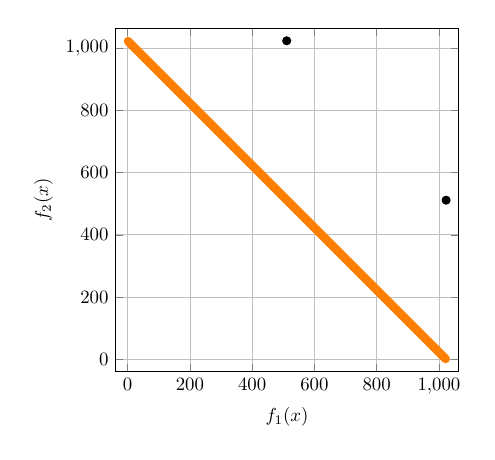
\begin{tikzpicture}[scale=0.68]
\begin{axis}[width=8cm, height=8cm,
    xlabel={$f_1(x)$},
    ylabel={$f_2(x)$},
%    legend style={at={(0.5,0.98)}, anchor=north},
    grid=major,
%    xtick={0,1,...,20},
    ymajorgrids=true,
    xmin=-40, xmax=1064,
    ymin=-40, ymax=1064,
    ]

\addplot[domain=1:1022,samples=1022,mark=*, color=orange] % non-Pareto
    plot[only marks]
    ({x},{2^10-1-x});
    
\addplot[mark=*, color=black, thick] % Pareto
    plot[only marks]
    coordinates {
    (2^10-1,2^9-1)
    (2^9-1,2^10-1)};
\end{axis}
\end{tikzpicture}
    \caption{Objective space}
\end{subfigure}
%
\begin{subfigure}[b]{0.58\textwidth}\centering        
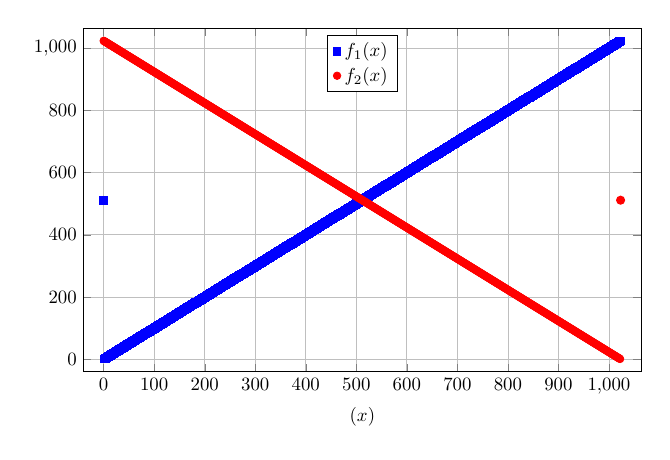
\begin{tikzpicture}[scale=0.68]
\begin{axis}[width=12cm, height=8cm,
    xlabel={$\Binval(x)$},
    %ylabel={Function Value},
    %title={Plots of $f_1(s)$ and $f_2(n-s)$ for $n=20$},
    legend style={at={(0.5,0.98)}, anchor=north},
    grid=major,
    %xtick={0,1,...,20},
    ymajorgrids=true,
    xmin=-40, xmax=1064,
    ymin=-40, ymax=1064,
]
\addplot[mark=square*, color=blue, thick, forget plot] % f_1
    plot[only marks]
    coordinates {
    (0,2^9-1)};
\addplot[domain=1:1023,samples=1023,mark=square*, color=blue]
    plot[only marks] 
    {x};
    \addlegendentry{$f_1(x)$}

\addplot[mark=*, color=red, thick, forget plot] % f_2
    plot[only marks]
    coordinates {
    (1023,2^9-1)};
\addplot[domain=0:1022,samples=1023,mark=*, color=red]
    plot[only marks] 
    {1023-x}; 
    \addlegendentry{$f_2(x)$}

\end{axis}
\end{tikzpicture}
    \caption{Phenotype--objective mapping}
\end{subfigure}
    \caption{$\OZBinval(x)$ with $n=10$.}\label{fig:ozbinval-10}
    \ifarxiv\else\Description{This figure illustrates \OZBinval with $n=10$.}\fi
\end{figure}


\begin{lemma}
\label{lem:binval-dominance}
\newedit{Let $f(x):=\OZBinval(x)$ and $F:=\{0^n,1^n\}$. Then:
\begin{enumerate}
    \item[(i)] $\forall x\in \{0,1\}^n \setminus F\colon f_1(x)+f_2(x)=2^{n}-1$,
    \item[(ii)] $\forall x,y\in \{0,1\}^n \setminus F, x\neq y\colon x \in \ndom{f}{y} \wedge y \in \ndom{f}{x}$,
    \item[(iii)] $\ndom{f}{1^n} = \{1^n\} \cup \{x \in \{0,1\}^n \mid x_1=0\}$,
    \item[(iv)] $\ndom{f}{0^n} = \{0^n\} \cup \{x \in \{0,1\}^n \mid x_1=1\}$,
    \item[(v)] $\Popt{f} = F$.
    %\item $\forall x \in \{0,1\}^n: \neg(1^n \succ x) \Leftrightarrow x_1=0$
    %\item $\forall x \in \{0,1\}^n: \neg(0^n \succ x) \Leftrightarrow x_1=1$
\end{enumerate}}

\end{lemma}
\begin{proof}
\newedit{Statement (i) holds because 
%for all $x\notin F\colon \OZBinval(x)=\BV(x)$, 
%thus $f_1(x)=\Binval(x)=\sum_{i\colon x_i=1} 2^{n-i}=\sum_{i} 2^{n-i} - \sum_{i\colon x_i=0} 2^{n-i} = 2^n -1 - \Binval(x \XOR 1^n)=2^n -1 -f_2(x)$.
$f(x)=\BV(x)=(\Binval(x),\Binval(x \XOR 1^n)$ for all $x\notin F$
%and since $x$ and $x\XOR 1^n$ are complement strings
thus 
%\dirk{We could also just say that bit $i$ contributes $2^{n-i}$ to either $f_1$ or $f_2$?}
bit $i$ contributes $2^{n-i}$ to either $f_1$ or $f_2$ exclusively and $f_1(x)+f_2(x)=\sum_{i=1}^{n}2^{n-i}=2^{n}-1$. 
Statement (ii) follows from (i) because assume without loss of generality that $f_1(x)>f_1(y)$, then $f_2(x)=2^n -1 - f_1(x) < 2^n -1 - f_1(y)=f_2(y)$, thus $x,y$ are incomparable.}

\newedit{It remains to show statement (iii), because then (iv) follows by symmetry. 
    Then the last statement (v) is a consequence of (iii) and (iv):
    % given that} 
%\[\newedit{(\{1^n\} \cup \{x \in \{0,1\}^n \mid x_1=0\}) \cap (\{0^n\} \cup \{x \in \{0,1\}^n \mid x_1=1\}) = F.}\]
%\dirk{Suggestion: we could expand this to
% 
\begin{align*}
\Popt{f} 
    =\;& \cap_{x\in\{0,1\}^n}\ndom{f}{x} = \ndom{f}{1^n} \cap \ndom{f}{0^n}\\
    =\;&  (\{1^n\} \cup \{x \in \{0,1\}^n \mid x_1=0\}) \cap (\{0^n\} \cup \{x \in \{0,1\}^n \mid x_1=1\})\\
    =\;& \{0^n, 1^n\} = F.
\end{align*}}
%}
%
%\newedit{Let $x \notin F$. If $f_1(x)>2^{n-1}-1$ then $f_2(x)\leq 2^{n-1}-1$ (since $f_1(x)+f_2(x)=2^n-1$) and hence, $x$ is dominated by $1^n$ due to $f(1^n)=(2^{n}-1,2^{n-1}-1)$. \dirk{Suggest to mention $f(1^n)$ to complete the argument.}\andre{done!} Otherwise, $x$ is dominated by $0^n$ (since $f_2(x) < 2^n-1$ and $f(0^n)=(2^{n-1}-1,2^n-1)$). We only show the second statement since the third follows by symmetry. For every $x \in \{0,1\}^n \setminus F$ we have $f_1(x) < 2^n-1$ since the binary value of $x \neq 1^n$ is smaller than $2^n-1$. If $x_1=0$ then $f_2(x) \geq 2^{n-1}$ since the binary value of $1^n \oplus x$ is at least $2^{n-1}$ in this case and hence, $1^n$ does not dominate $x$. If $x_1=1$ then $f_2(x) \leq 2^{n-1}-1$ and hence, $1^n$ dominates $x$. \andre{I am more compact and put all the results in this lemma. Please check.}}
%
%\cuong{The above looks confusing to me, so I try to formulate it like this}. 
\newedit{We thus prove (iii) and note that $1^n \in \ndom{f}{1^n}$ by definition. Furthermore, $f(1^n)=(2^n-1, 2^{n-1}-1)$ and $f(0^n)=(2^{n-1}-1, 2^n-1)$, so $0^n$ and $1^n$ are incomparable and $0^n \in \ndom{f}{1^n}$. What is left to show is that for all $x\notin F\colon$ $x\in \ndom{f}{1^n}$ if and only if $x_1=0$. First note that $f_1(x)<2^n - 1=f_1(1^n)$ since this $f_1$-value of $2^n - 1$ can only be obtained from $1^n \neq x$. For the case $x_1=0$, notice similarly that $f_1(x)\leq 2^{n-1}-1$, thus by statement (i) we get $f_2(x)=2^n-1-f_1(x)\geq 2^n-1-(2^{n-1}-1)=2^{n-1}>f_1(1^n)$, so 
%$1^n$ does not dominate $x$, or equivalently 
$x\in \ndom{f}{1^n}$.
In the other case of $x_1=1$, we get $f_1(x)\geq 2^{n-1}$ and again by (i) $f_2(x)=2^n-1-f_1(x)\leq 2^{n-1} - 1=f_1(1^n)$, so $1^n \succ x$ and, equivalently, $x\notin \ndom{f}{1^n}$.}
\end{proof}

\newedit{From this lemma, we can deduce that \OZBinval is \ineff{$1$}{$1$} because $\hdist(0^n,0^{n-1}1)=1$ and $0^{n-1}1 \in \ndom{\OZBinval}{1^n}$. The bound provided by Theorem~\ref{thm:gsemo} is therefore too weak to show the difficulty that this function imposes on (G)SEMO. In fact, the algorithms fail for the completely opposite reason to what we have discussed so far: they keep too many solutions.}

\subsection{\newedit{(G)SEMO performs a blind random search on \OZBinval}}\label{sec:gsemo-ozbinval}
\newedit{
Note that GSEMO keeps all non-dominated solutions and therefore it keeps all distinct solutions ever seen before a Pareto-optimal solution is generated. This behaviour indicates that GSEMO performs a somewhat blind random search and hence needs at least $\Omega(2^{n})$ fitness evaluations in expectation to find one Pareto optimal point since the proportion of Pareto-optimal points is only a fraction of $2/2^n = 1/2^{n-1}$. We can even formulate this result for a large class of mutation operators which meet the following property.}
%Note that all solutions which are not Pareto optimal are pairwise incomparable since for each such $x \in \{0,1\}^n \setminus \{x \mid \LO(x)+\TZ(x)=n\}$ we have $x_1+x_2=\sum_{i=1}^n2^{i-1} = 2^n-1$ and the value of the first objective of two non-Pareto-optimal $x,y$ differs. Note that GSEMO keeps all non-dominated solutions and therefore, all solutions ever seen before a Pareto-optimal solution is generated. This behaviour indicates that GSEMO needs at least $2^n$ fitness evaluations in expectation to find one Pareto optimal point which we will prove in the following. 
%\begin{lemma}
%\label{lem:GSEMO-inef-Binval}
%   The expected number of fitness evaluations required for (G)SEMO on \OZBinval  is dominated by a geometric distribution with parameter $2^{-n+1}=2^{-\Omega(n)}$. In other words, GSEMO requires at least $2^{n-1}$ expected fitness evaluations to optimize \OZBinval.
%\end{lemma}
%\dirk{Can we use symmetry to derive a much shorter proof? Or cite black-box complexity results? These might also cover arbitrary unbiased mutation operators.}
%\begin{proof}
%    Let $F:=\{0^n,1^n\}$ and $T$ be a random variable with $T:=\inf\{t \in \mathbb{N} \mid P_t \cap F \neq \emptyset\}$. Note that $T$ is stochastically dominated by the optimization time, i.e. the time until (G)SEMO covers the whole Pareto front. We consider a variant (G)SEMO' of (G)SEMO which starts with one individual $x$ chosen uniformly at random (i.e. $P_0'=\{x\}$), and in each iteration selects a parent $z$ uniformly at random from its current population $P_t'$, applies standard bit mutation to $z$ in order to create an offspring $y$ and adds $y$ to $P_t'$ if there is no $y' \in P_t'$ with $y'=y$ and otherwise %replaces $y'$ 
%    discards $y$ (i.e. duplicates will be avoided). Note that (G)SEMO' has no stopping criterion and may add dominated solutions to $P_t'$. However, for $T':=\inf\{t \in \mathbb{N} \mid P_t' \cap F \neq \emptyset\}$ we have $T=T'$ since (G)SEMO on $\OZBinval$ behaves in the same way as (G)SEMO', as long as no Pareto-optimal individual is created since all non Pareto-optimal solutions are pairwise incomparable. Hence, our aim is to show that $T'$ %is stochastically dominated 
%    can be seen as a geometrically distributed random variable with parameter $2 \cdot 2^{-n} = 2^{-n+1}$. Let $x_1, x_2, \ldots$ be the sequence of individuals generated by (G)SEMO'. %Note that $x_1, \ldots ,x_T$ tracks all individuals ever generated by (G)SEMO' and hence, 
%    \cuong{I am not sure if introducing (G)SEMO' is required. I think we only need to define $T'$ for GSEMO, and it is clear that $T'\leq T$ and before this stopping time $T'$ all solutions are inserted in the population without removing those already exist.}
%    \dirk{Alternatively, we could consider a fitness function $(\textsc{BinVal}(x), \textsc{BinVal}(x \oplus 1^n))$ and the original GSEMO.}
%    Note that in this sequence duplicates may occur (for example if (G)SEMO' creates an individual in an iteration $t$ which is already created in a previous iteration $t'<t$). We show by an induction on $j$ that for all search points $y \in \{0,1\}^n$ we have $\Pr(x_j = y) = 2^{-n}$. 
%    The probability that $x_1 = y$ for any search point $y \in \{0,1\}^n$ is $2^{-n}$ since (G)SEMO' initializes an individual uniformly at random. Suppose that the claim holds for iteration $1 \leq j$. 
%    Assume that in iteration $j+1$ for a given $w \in \{0,1\}^n$ the mutation operator $\text{mut}_w$ is applied to the parent $z \in P_t'$ which creates $x_{j+1}=z \oplus w$. Then by the law of total probability since the parent $z$ is chosen uniformly at random from $P_t'$
%    \cuong{In the writing below, I would suggest to write what the algorithm does in the subscript of the probability, something like $\Pr_{x_{j+1}\sim \text{mut}_w(z)}(x_{j+1}=y)$, instead of the condition to reduce the cumbersomeness. Also do we have any requirement on how the algorithm can choose $w$? I do not see this $w$ is used in further calculations.}
%    \begin{align*}
%    \Pr(x_{j+1}&=y \mid \text{mut}_w) = \sum\nolimits_{z \in P_t'} \frac{1}{\vert{P_t'}\vert}\Pr(x_{j+1}=y \mid \text{mut}_w,z).
%    \end{align*}
%    We can further write by the law of total probability (where ''$z=x$'' denotes the event that the parent $z$ coincides with a specific $x \in \{0,1\}^n$)
%    \begin{align*}
%    &= \sum\nolimits_{z \in P_t'} \sum\nolimits_{x \in \{0,1\}^n} \frac{1}{\vert{P_t'}\vert}\Pr(x_{j+1}=y \mid \text{mut}_w,z,z=x) \Pr(z=x).
%    \end{align*}
%    Since $\Pr(z=x)=1/2^n$ by the inductive hypothesis, and $x_{j+1} = x \oplus w$ under the given conditions (since $\text{mut}_w$ is applied to the parent $z$ and $z$ coincides with $x$), we further obtain
%    \begin{align*}
%    &= \sum\nolimits_{z \in P_t'} \frac{1}{2^n}\frac{1}{\vert{P_t'}\vert} \sum\nolimits_{x \in \{0,1\}^n} \Pr(x_{j+1}=y \wedge x_{j+1} = x \oplus w \mid \text{mut}_w,z,z=x).
%    \end{align*}
 %   The condition $x_{j+1}=y \wedge x_{j+1} = x \oplus w$ is only fulfilled if $x=y \oplus w$ (since then $x \oplus w = y \oplus w \oplus w = y$ and otherwise $x \oplus w \neq y$) which implies
%    \begin{align*}
%    &= \sum\nolimits_{z \in P_t'} \frac{1}{2^n}\frac{1}{\vert{P_t'}\vert} \Pr(x_{j+1}=y \mid \text{mut}_w,z,z=y \oplus w)\\
%    &= \sum\nolimits_{z \in P_t'} \frac{1}{2^n}\frac{1}{\vert{P_t'}\vert} = \frac{1}{2^n}.
%    \end{align*}
    %&= \sum\nolimits_{z \in P_t}\frac{1}{2^n}\frac{1}{\vert{P_t}\vert}\sum\nolimits_{x \oplus w \in \{0,1\}^n}\Pr(x_{j+1}=x \cap x_{j+1} = y \mid \text{mut}_w,z,z=x \oplus w)\\
    %&= \sum\nolimits_{z \in P_t}\frac{1}{2^n}\frac{1}{\vert{P_t}\vert}\sum\nolimits_{x \oplus w \in \{0,1\}^n}\Pr(x_{j+1}=x \cap x_{j+1} = y \mid \text{mut}_w,z,z=x \oplus w)\\
    %&= \sum\nolimits_{z \in P_t}\sum\nolimits_{x \in \{0,1\}^n} \frac{1}{\vert{P_t}\vert}\Pr(z=x \oplus w \mid \text{mut}_w,z,z=x \oplus w)
    %Since this result is independent of the used mutation operator $\text{mut}_w$ used in iteration $j+1$ we see (again by the law of total probability) $\Pr(x_{j+1}=y) = 1/2^n$ which concludes the induction. \\
    %Hence, we obtain for every iteration $j$ by a union bound on $|F|$ that $\Pr(x_j \in F) = 2/2^n=1/2^{n-1}$ which concludes the proof.
    %\cuong{You need to do the union bound on $j$ too, otherwise the statement is too strong: essentially you are saying that the probability of finding a Pareto optimal solution is $1/2^{n-1}$ at any iteration $j$, in reality this probability changes if $j$ is too large like $j=4^n$. In fact, your computed probability is conditional, for it to hold at iteration $j$ no Pareto-optimal point should have found yet in all the $j-1$ previous iterations.} 
%\end{proof}}

    We say that a mutation operator $\mathrm{mut}$ is invariant to bit values if for all 
    $x, y, a \in \{0, 1\}^n$ 
    it holds $\Prob{\mathrm{mut}(x) = y} = \Prob{\mathrm{mut}(x \oplus a) =  y \oplus a}$.
    This property means that there is no bias for specific bit values. All unary unbiased operators in the sense of~\citet{Lehre2012} meet this property.  This includes 1-bit flips, standard bit mutation and heavy-tailed mutation operators~\cite{Doerr2017-fastGA}.

    The following theorem applies to GSEMO using any mutation operator invariant to bit values. This includes the classical GSEMO with standard bit mutations and SEMO using 1-bit flips. 
\begin{theorem}
\label{thm:GSEMO-inef-Binval}
   Consider GSEMO using an arbitrary mutation operator invariant to bit values.
   The number of 
   fitness evaluations 
   required for GSEMO on \OZBinval to find the Pareto front 
   %is stochastically dominated by 
   stochastically dominates
   a uniform distribution on $\{1, \dots, 2^{n-1}\}$. Consequently, GSEMO requires at least 
   %$2^{n-2}-1/2$ 
   \newedit{$2^{n-2}+1/2$}
   fitness evaluations in expectation to find a Pareto-optimal search point on \OZBinval.
\end{theorem}
\begin{proof}
    \newedit{
    %We first consider the search dynamics of 
    The algorithm 
    %on the function 
    %\[
    %    \BV(x) \coloneqq (\Binval(x), \Binval(x \oplus 1^n)), 
    %\]
    %on which all search points $x \neq y$ are incomparable. Note that GSEMO: 
    %it 
    behaves identically on \OZBinval and \BV up to the point a Pareto-optimal search point is found.}
    The search process of GSEMO on \BV can be described using a family tree $\tree$ as follows. In a family tree (first studied in the context of runtime analysis of evolutionary algorithms by~\citet{Witt2006}), every node represents an individual and edges represent parent-child relationships.
    We say that a node is \textit{alive} at time~$t$ if it is contained in~$P_t$.
    
    Now GSEMO first creates an initial search point $x_0 \in \{0, 1\}^n$ uniformly at random. 
    This search point represents the root of the family tree. In every subsequent generation~$t$ GSEMO picks a node uniformly at random from all alive nodes. Let $x_t$ be the corresponding search point, then GSEMO applies some mutation operator $\mathrm{mut}$ invariant to bit values to~$x_t$, and adds a new child node to the parent node that represents the generated offspring, $y_t = \mathrm{mut}_t(x_t)$.

    We argue that, at any point in time~$t$, all nodes in $\tree$ can be described as a (meta-)mutation of the initial search point~$x_0$. More specifically, every search point $x$ in the tree can be described as $x = x_0 \oplus a_x$, where $a_x \in \{0, 1\}^n$ is a mask that describes which bits were flipped an odd number of times in the lineage that evolved $x$ from $x_0$. For $x^0$ itself we have $x_0 = x_0 \oplus 0^n$, hence we choose $a_{x_0} \coloneqq 0^n$. Now consider a generation creating an offspring $y$ from a parent $x$ and assume that $x$ has a mask $a_x$, \ie, $x = x_0 \oplus a_x$. Let $m \in \{0, 1\}^n$ be a mask describing which bits were flipped in $\mathrm{mut}(x)$: $m_i = 1$ if and only if bit $i$ was flipped during this mutation. Then we have $y = x \oplus m$ and, consequently, $y = (x_0 \oplus a_x) \oplus m = x_0 \oplus (a_x \oplus m) = x_0 \oplus a_y$ when choosing $a_y \coloneqq a_x \oplus m$.
    \newedit{In the original family tree method \cite{Witt2006}, each node is labelled with its creation time and the associated search point. In our approach, we replace the search point $x$ with its mutation mask $a_x$, since given $x_0$ and our labelled tree, we can recover the other labelled tree. We can further detect, at any time, which nodes are alive by looking at the current labels. That is, a node labelled $(t,a_x)$ is alive if and only if there exists no node in the tree with label $(t',a_x)$ where $t'>t$.}

    Using this perspective, we apply the method of deferred decisions~\cite[Section~3.5]{Motwani1995}: we consider GSEMO starting with a random string $x_0$ and we only reveal the random choice of~$x_0$ at a later stage. The above arguments
    %on masks 
    %and the fact that 
    %on \BV all new search points are included in the population 
    % \newedit{at any time, we can detect which nodes are alive by looking at the current labels, \ie a node labelled $(t,a_x)$ is alive if and only if there exists no node in the tree with label $(t',a_x)$ where $t'>t$,}
    show that we can apply uniform parent selection and our mutation operator without the need to know the values of~$x_0$.
    %\cuong{Ah, it is not precise that all nodes are alive at any time $t$, some are not if their creation time is $t'$ and a copy of it appears at time $t''>t'$. But this is fine, we can determine the alive status easily with the masks, without knowing $x_0$. I will try to fix this.}
    %\cuong{Done.}

    Consider GSEMO after $t$ generations and let $\tree_t$ be the family tree at time~$t$. 
    %contains $|\tree_t|$ mutually different search points \cuong{We should drop this assumption, see below}. 
    Now we fix a target search point~$z$, which we will choose as $0^n$ and $1^n$, respectively. Then the following holds.
    For every search point $x \in \tree$, we have $\Prob{x = z} = \Prob{(x_0 \oplus a_x) = z} = \Prob{x_0 = (a_x \oplus z)} = 1/2^{n}$. 
    %Since these events for different search points $x \neq x'$ are disjoint, $\Prob{z \in \tree_t} = |\tree_t|/2^n$ \cuong{We do not need them to be disjoint right? Since we can write $\Prob{z \in \tree_t} \leq |\tree_t|/2^n$ as a union bound on the number of nodes of the tree.}.
    By a union bound \newedit{on the numbers of Pareto-optimal search points and of nodes in the tree},
    \[
        \Prob{\{0^n, 1^n\} \cap \tree_t \neq \emptyset} \le \Prob{0^n \in \tree_t} + \Prob{1^n \in \tree_t} \le \frac{2|\tree_t|}{2^n} 
        \newedit{=\frac{2(t+1)}{2^n}.}
        %\le \frac{2t}{2^n}.
    \]
    Since GSEMO behaves as on $\BV$ up to the point $0^n$ or $1^n$ are discovered, if $T$ is 
    the first 
    %point in time 
    \newedit{generation} 
    in which the Pareto front is found, the algorithm has evaluated $T+1$ search points and
    \[
        \Prob{T+1 \le t} = \Prob{T \le t-1} \le \frac{\newedit{t}}{2^{n-1}}.
    \]
    The formula to the right equals the probability $\Prob{U \le t}$ when $U$ is chosen uniformly at random from $\{1, \dots, 2^{n-1}\}$. Hence, $T+1$ 
    %is stochastically dominated by~$U$.
    \newedit{stochastically dominates~$U$}. 
    The second statement follows from 
    \[
        \E{T}\geq \E{U}= \frac{1}{\newedit{2^{n-1}}} \sum_{i=1}^{2^{n-1}} i = \frac{2^{n-1}(2^{n-1}+1)}{2 \cdot 2^{n-1}}
        %\frac{2^{n-1}+1}{2} 
        =
        2^{n-2}+\frac{1}{2}.
    \]
    %\newedit{and noting that at a generation $T\geq 0$ the algorithm has performed $1+T$ fitness evaluations.}
\end{proof}

\subsection{\newedit{Popular EMOAs are efficient on \OZBinval}}\label{sec:nsga-smsemoa-ozbinval}

%\newedit{
%To be able to show that the other three algorithms are able to optimise \OZBinval in polynomial expected time, we need the following notion of LO/LZ-monotonicity. This is similar to the notion of 0/1-monotonicity in the context of \OTZTfull considered earlier.
%}
%\newedit{
%\begin{definition}\label{def:LO/LZ-monotone}
%Consider algorithm $\mathcal{A}$ optimising a $d$-objective function 
%$f\colon\{0,1\}^n \rightarrow \Z^d$ by evolving a population $P_t$ of search points 
%at each of its iteration $t\geq 0$. 
%$\mathcal{A}$ is called \emph{\LOLZmonotone} on $f$ if both of the following statements 
%hold: 
%\begin{itemize}
%\item $\exists x \in P_{t+1}\colon \LO(x) \geq \max\{\LO(z) \mid z \in P_t\}$,
%\item $\exists y \in P_{t+1}\colon \LZ(y) \geq \max\{\LZ(z) \mid z \in P_t\}$.
%\end{itemize}
%\end{definition}
%}

\newedit{In this subsection we prove that \nsga, \nsgaiii as well as SMS-EMOA can optimize $f:=\OZBinval$ efficiently. 
%In case of \nsga and \nsgaiii, we apply the level-based theorems for runtime analysis of MOEAs from~\cite{LevelBasedMOEAs} to our situation. 
To this end, we apply the level-based theorems for runtime analysis of MOEAs from~\cite{LevelBasedMOEAs} to our situation. At first we recall the necessary concepts. A partition $A_0, \ldots , A_k$ of the search space %such that all $A_i$ are non-empty \andre{why do we need that they are non-empty? I would drop that and I need this also for my proof below.} 
is called \emph{level partition} and an algorithm $\mathcal{A}$ evolving populations $P_0,P_1, \ldots$ is called \emph{level-monotone with respect to} $A_0, \ldots , A_k$ if $\ell(P_{t+1}) \geq \ell(P_t)$ where $\ell(P_t)$ denotes the highest index of the level set reached by the population $P_t$ so far, i.e. $\ell(P_t):=\max\{i \mid P_t \cap A_i \neq \emptyset\}$. 
}

\dirk{Should this come after the level-based theorem?}\newedit{\dirk{Added some text:} There are usually different ways to choose a level partition. Sometimes it can be useful to use a coarse-grained level partition to reduce the number of levels. The following lemma states that if an algorithm $\mathcal{A}$ is level-monotone for a fine-grained level partition $B_0, \dots, B_m$, then it is also level-monotone for a level partition~$A_0, \dots, A_k$ that results from merging neighbouring levels in~$B_0, \dots, B_m$.
%, if the level sets of $A$ are supersets of level sets of~$B$.
\begin{lemma}\label{lem:partition-finer}
Let $A_0, \ldots , A_k$ and $B_0, \ldots B_m$ be two level partitions with $k \leq m$ such that there are $0 =\ell_0< \ldots < \ell_k = m$ with $B_{\ell_j}, \ldots ,B_{\ell_{j+1}-1} \subset A_j$ for $j \in \{0,\ldots , k-2\}$ and $B_{\ell_{k-1}}, \ldots ,B_{\ell_k} \subset A_k$. In other words, $B_0, \ldots , B_m$ is \emph{finer} than $A_0, \ldots , A_k$. \dirk{Would to it be easier to say that $A_i$ is a union of neighbouring $B$-sets? See text above.} If an algorithm $\mathcal{A}$ is level-monotone for $B_0, \ldots , B_m$ then it is also level-monotone for $A_0, \ldots , A_k$.
\end{lemma}
\begin{proof}
    Suppose that the best level of $\mathcal{A}$ with respect to $A_0, \ldots , A_m$ in iteration $t$ is $A_j$. Then the current best level of $\mathcal{A}$ with respect to $B_0, \ldots , B_m$ in iteration $t$ is $B_i$ where $i \in \{\ell_j, \ldots ,\ell_{j+1}-1\}$ if $0\leq j \leq k-2$ or $i \in \{\ell_{k-1}, \ldots ,\ell_k\}$ otherwise. Due to level-monotonicity of $\mathcal{A}$ with respect to $B_0, \ldots , B_m$ the best level of $\mathcal{A}$ with respect to $B_0, \ldots , B_m$ in iteration $t+1$ is $B_{i'}$ with $i' \geq i$ and therefore $A_{j'}$ with respect to $A_0, \ldots , A_k$ for $j' \geq j$. Hence, $\mathcal{A}$ is also level-monotone with respect to $A_0, \ldots , A_k$.   
\end{proof}}

\newedit{The level-based theorem is formulated as follows where $A_{>m}:=\bigcup_{i=m+1}^k A_i$ for $0 \leq m \leq k-1$.
\begin{theorem}(\cite[Theorem~6]{LevelBasedMOEAs})
\label{thm:extended-fitness-level-result}
    Consider a level partition $A_0, \dots, A_k$ and a level-monotone algorithm $\mathcal{A}$ evolving populations $P_0, P_1, \dots$ of cardinality $\mu$.
    Assume that $\mathcal{A}$ creates $\lambda$ offspring by using 
    %fair selection (where $\lambda = \mu$) or 
    some independent parent selection where a parent in $A_{\ell(P_t)}$ is chosen with probability at least $|A_{\ell(P_t)}\cap P_t|/|P_t|$.
    %\dirk{The latter condition is true for NSGA-II with tournament selection. If it was false it would mean that selection would favour parents that are worse in their primary fitness criterion!}
    %
    For $0 \le i \le k-1$ let $s_i \in (0, 1]$ be a lower bound on the probability of creating a search point in $A_{>\ell(P_t)}$ when selecting a parent in $A_{\ell(P_t)}$. 
    Let $T$ denote the random number of evaluations made until the last level $A_k$ is reached. Then, for every initial population\footnote{The fact that the theorem applies to arbitrary initial populations was not made explicit in~\cite{LevelBasedMOEAs}, but it is evident from the proofs.} of size~$\mu$, the following statements hold. \dirk{Added a statement on arbitrary initial populations and a footnote explaining this.}
    \begin{itemize}
        \item[(1)]
        \[
            \E{T} \le \lambda k + \mu\sum_{i=0}^{k-1} \frac{1}{s_i}.
        \]
        (For $\lambda=1$ the summand $\lambda k$ can be dropped.)
        \item[(2)] $T$ is stochastically dominated by \newedit{a sum of independent random variables:}
        \[
            \lambda\sum_{i=0}^{k-1} \mathrm{Geom}(1-(1-s_i/\mu)^\lambda).
        \]
        \item[(3)] For every $\delta \ge 0$, 
        \[
            \Prob{T >  \lambda k + \mu\sum_{i=0}^{k-1} \frac{1}{s_i} + \delta\lambda}
            \le e^{-(\delta/4)\min\{\delta/s, h\}}
        \]
        where $h \coloneqq \min\{1-(1-s_i/\mu)^\lambda \mid 0 \le i \le k-1\}$ and $s \coloneqq \sum_{i=0}^{k-1}\frac{1}{(1-(1-s_i/\mu)^\lambda)^2}$. 
    \end{itemize}
\end{theorem}
%If the level partition $A_1, \ldots ,A_k$ is chosen such that $A_k$ contains only Pareto-optimal search points, then $T$ is also the random number of evaluations made until the Pareto front is reached.
For our purposes we consider for $f:=\OZBinval$ the following two different level partitions for $i \in \{1,2\}$. Let $C_0^i, \ldots ,C_n^i$ with $C_j^1:=\{x \in \{0,1\}^n \mid \LO(x)=j\}$ and $C_j^2:=\{x \in \{0,1\}^n \mid \LZ(x)=j\}$. Note that $C_{n}^1=\{1^n\}$ and $C_{n}^2=\{0^n\}$. Therefore, the time required by a multi-objective evolutionary algorithm $\mathcal{A}$, which is level-monotone with respect to $C_0^i, \ldots , C_n^i$, on $f$ to find $1^n$ or $0^n$ corresponds to the time $T$ from Theorem~\ref{thm:extended-fitness-level-result} it takes to reach the last level, $C_n^1$ or $C_n^2$, respectively.
%For our proof we %for a bi-objective objective function $f:\{0,1\}^n \to \mathbb{N}$ and both objectives $i \in \{1,2\}$ 
%consider for $f:=\OZBinval$ the level-partition $B_1^i, \ldots , B_{2^n-1}^i$ where $B_j^i:=\{x \in \{0,1\}^n \mid f_i(x)=j\}$ for $j \in \{0, \ldots , f_{\max}\}$ and $i \in \{1,2\}$ (compare with Lemma~14 in~\cite{LevelBasedMOEAs}).
%However, in~\cite{LevelBasedMOEAs} it is shown that \nsga for $\mu \geq 3$ and \nsgaiii for $\mu \geq |\refer|$ with $\{(0,1),(1,0)\} \subset \refer$ are level-monotone with respect to $B_1^i, \ldots , B_{g_{\max}}^i$ for any bi-objective function $g:\{0,1\}^n \to \mathbb{N}^2$ (compare with Lemma~14 in~\cite{LevelBasedMOEAs}). 
Hence, our aim is to show that \nsga, \nsgaiii and SMS-EMOA on $f$ are level-monotone with respect to $C_0^i, \ldots ,C_n^i$ and then we will directly apply Theorem~\ref{thm:extended-fitness-level-result} on all three algorithms, using appropriate probability bounds $s_i$, to derive the desired runtime bounds.}

\newedit{\begin{lemma}
\label{lem:algorithms-LO/LZmonotone}
    Let $i \in \{1,2\}$. The following algorithms using standard bitwise mutation or the local mutation as a variation operator on $f:=\OZBinval$ are level monotone with respect to $C_0^i, \ldots , C_n^i$.
    \begin{itemize}
       \item[(i)] \nsga with $\mu \geq 3$,
      \item[(ii)] \nsgaiii with $\mu \geq |\refer|$ and $\{(0,1),(1,0)\} \subset \refer$,
        \item[(iii)] SMS-EMOA with $\mu \geq 2$ and using $h \preceq (-2^{2n-2},-2^{2n-2})$ for its reference point.
    \end{itemize}
\end{lemma}
\begin{proof}
    We show that all three algorithms in their appropriate setting are level monotone with respect to $C_0^1, \ldots , C_{n}^1$. Let $P_t$ be a population. If $\ell(P_t)=0$ then the statement clearly follows for all three algorithms since the \LO-value of a search point is non-negative. Now suppose that $\ell(P_t)>0$ and let $x \in P_t$ be a solution with $\LO(x)=\ell(P_t)=:k$. Then $f_1(x) \geq 2^{n-1} + \ldots + 2^{n-k}$ and for every other solution $y$ with $f_1(y) \geq 2^{n-1} + \ldots + 2^{n-k}$ we also have $\LO(y) \geq k$ (since $f_1(0^n)=2^{n-1}-1$ and for $y \neq 0^n$ the first objective represents the binary value of $y$ and hence, a $y$ with $\LO(y) < k$ fulfills $f_1(y) < 2^{n-1} + \ldots + 2^{n-k}$). Hence, for all three algorithms we show that there exists a search point $y \in P_{t+1}$ such that $f_1(y) \geq 2^{n-1} + \ldots + 2^{n-k}$, particularly that they are all level monotone with respect to the level partition $B_0^1, \ldots , B_{2^n-1}^1$ defined as $B_i^1:=\{x \mid f_1(x)=i\}$. Then Lemma~\ref{lem:partition-finer} implies level monotonicity of $C_0^1, \ldots , C_n^1$.
    In Lemma~14 in~\cite{LevelBasedMOEAs} it has already been shown\cuong{Which theorem/lemma was that? We need a precise citation.}\andre{done!} that \nsga and \nsgaiii are level monotone with respect to this partition\footnote{In case of \nsga the population size is chosen to be $\mu \geq 2$ there, but this is due to the stable sorting algorithm used there for calculating the crowding distance. Here we do not make any assumption on sorting in this context.}. 
    Hence, it is left to show (iii).%This can be achieved by showing that the maximum fitness in the first objective cannot decrease (i.e. $\max_{x \in P_{t}}f_1(x) \leq \max_{x \in P_{t+1}}f_1(x)$) which we will do in the following.
    \dirk{Should we put this in a separate lemma? Might be of independent interest. Then the reference point could be something like $(-f_{\max}^2, -f_{\max}^2)$.}
    \andre{Good point, but I would leave that for our journal extension of the PPSN paper. There it is more compatible with the content.}\\
    % Then $j \geq 2^{n-1}$ and therefore $2^n-1-j = \min\{f_2(x) \mid x \in P_t\}$.\\
    %(i): Let $R_t$ be a joint population created from $P_t$. Since $P_t \subset R_t$, it is enough to show that one individual from $R_t$ with maximum fitness is taken into $P_{t+1}$. Let $y \in R_t$ be with maximum possible $f_1$-value. Note that $y$ is non-dominated and hence $y \in F_{t+1}^1$. If $|F_{t+1}^1| \leq \mu$, all solutions from $F_{t+1}^1$ (including $y$) will be taken into $P_{t+1}$ and the property follows. If $\ell:=|F_{t+1}^1| > \mu$ then $F_{t+1}^1=F_{t+1}^{i^*}$ and the ranking of the solutions uses the crowding distance calculation. Let $(S_1[1], \ldots , S_1[\ell])$ be the sorting of all individuals from $F_{t+1}^1$ with respect to the first objective and $(S_2[1], \ldots , S_2[\ell])$ the sorting with respect to the second one (both in decreasing order). Note that the solutions of the set $I:=\{S_1[1],S_1[\ell],S_2[1],S_2[\ell]\}$ have infinite crowding distance and, consequently, they are top ranked. We also have $f_1(S_1[1]) \geq f_1(S_2[\ell])$ and $f_2(S_1[1]) \geq f_2(S_2[\ell])$ which yields $f(S_1[1]) = f(S_2[\ell])$ since $S_1[1]$ and $S_2[\ell]$ are non-dominated. This implies that in any three solutions from $I$ there is always at least one with fitness $f(S_1[1])$, i.e. with maximum fitness in the first objective among all individuals from $R_t$. This individual will be taken into $P_{t+1}$.\\  
    %(ii): Let $R_t$ be a joint population created from $P_t$ and let $y \in R_t$ be a solution with maximum $f_1$-value. Note that $y \in F_{t+1}^1$ and, as in the previous part (i), we can assume that $|F_{t+1}^1| > \mu$. %Note that $x \in F_{t+1}^1$. If $|F_{t+1}^1| \leq \mu$ all solutions from $F_t^1$ (including $x$) will be taken into $P_{t+1}$ and the property follows. 
    %Then $F_{t+1}^1=F_{t+1}^{i^*}$ and the ranking of the solutions uses the \textsc{Niching} procedure from Algorithm~\ref{alg:ref-points}. For the normalization we have $z_1^{\min}=\min\{f_1(x) \mid x \in F_{t+1}^1\}$ and $z_2^{\min}=\min\{f_2(x) \mid x \in F_{t+1}^1\}$. Note that $y$ has minimum $f_2$-value among all individuals from $F_{t+1}^1$ (otherwise it dominates another $z \in F_{t+1}^1$).
    %Consequently, the normalization on $x$ gives $f^n(x)=(a,0)$ for $a \geq 0$. If $a=0$ then $f_1(y) = z_1^{\min}$ and hence all individuals from $F_t^1$ have the same fitness in the first objective, i.e. the same \LO-value. Then it is obvious that this \LO-value does not change between $R_t$ and $P_{t+1}$. Otherwise, $a>0$ and the distance between $f^n(x)$ and the reference ray $(1,0)$ is zero, which is smallest possible. Thus all points $z$ with normalized $f^n(z)=(a,0)$ are associated to $(1,0)$. All other points $w \in F_t^1$ with not-maximum $f_1$-value have larger $f_2$-values than $z$ and hence, $f^n_2(w)>0$. Hence, they have larger distance to the reference ray $(1,0)$ than $y$. Since Algorithm~\ref{alg:ref-points} prefers reference points which the smallest niche count so far, every reference point keeps at least one solution associated to it with the smallest distance. Therefore, one solution from $R_t$ with the maximum $f_1$-value survives.\\
    (iii): Let $R_t$ be a joint population created from $P_t$ (i.e. $|R_t| \geq 3$) and let $y \in R_t$ be a solution with maximum $f_1$-value. Note that $y \in F_{t+1}^1$. If there is $z \in R_t \setminus F_{t+1}^1$ then $y$ survives since only one individual from the layer below $F_{t+1}^1$ will be deleted. If there are two individuals with maximum $f_1$-value then one of them survives. Hence, suppose that $R_t = F_{t+1}^1$ and there is exactly one individual $y$ with maximum $f_1$-value in $R_t$. Then all other individuals have an $f_1$-value of at most $f_1(y)-1$ and hence, we obtain
    \begin{align*}
    \hv(F_{t+1}^1) &\geq \hv(F_{t+1}^1 \setminus \{y\})+\mathcal{L}(\{(a_1,a_2) \in \mathbb{R}^2 \mid f_1(y)-1<a_1\leq f_1(y), h_2 \leq a_2 \leq 0\}) \\
    &= \hv(F_{t+1}^1 \setminus \{y\})+h_2.
    \end{align*}
    In other words, the hypervolume contribution of $y$ is at least $h \geq 2^{2n-2}$.  
    So suppose that there are $z,w \in F_1^t$ with $\{y,z,w\} \subset F_1^t$ and $f_1(y)>f_1(w)>f_1(z)$ (i.e. $f_2(y)<f_2(w)<f_2(z)$ since $y,z,w$ are non-dominated). Then the hypervolume contribution of $w$ is at most (no matter if $F_t^1 \setminus \{y,z,w\} = \emptyset$ or not since removing search points from $F_t^1 \setminus \{y,z,w\}$ may only increase the hypervolume contribution of $w$)
    \begin{align*}
    (f_1(w)-f_1(z))(f_2(w)-f_2(y)) &\leq f_1(w)f_2(w) = f_1(w) \cdot (2^n-1 - f_1(w))\\
    &< f_1(w) \cdot (2^n - f_1(w)) \leq (2^n/2)^2 = 2^{2n-2}
    \end{align*}
    which shows that $w$ has a smaller hypervolume contribution than $y$. Thus, $y$ is guaranteed to survive, implying level-monotonicity with respect to $B_0^1, \ldots , B_{2^n-1}^1$ of SMS-EMOA on $f$.\\
    By a completely symmetric argument one can obtain level monotonicity of all three algorithms with respect to $B_0^2, \ldots , B_{2^n-1}^2$ where $B_j^2:=\{x \mid f_2(x)=j\}$ which implies level monotonicity with respect to $C_0^2, \ldots , C_n^2$ by Lemma~\ref{lem:partition-finer}. %In case of \nsga and \nsgaiii the former is also shown in~\cite{LevelBasedMOEAs}. %since one can show in a similar way that the maximum fitness in the second objective (reflecting the maximum \LZ-value) cannot decrease.
\end{proof}}

\newedit{
Finally, we can apply Theorem~\ref{thm:extended-fitness-level-result} and obtain the following results on the expected runtime.}

\newedit{\begin{lemma}
\label{lem:Algos-eff-Binval}
   For every initialization, \nsga with $\mu \geq 3$, \nsgaiii with $\mu \geq |\refer| \geq 2$ and SMS-EMOA using standard bitwise mutation or local mutation as a variation operator cover the whole Pareto front of \OZBinval in $6\mu n^2$ fitness evaluations with probability $1-e^{-\Omega(n)}$. The expected number of fitness evaluations is $O(\mu n^2)$.
\end{lemma}
}

\begin{proof}
\newedit{We show that starting with any initial population both algorithms find $1^n$ in $6\mu n^2$ fitness evaluations with probability $1-e^{-\Omega(n)}$. The analogous result for $0^n$ can be obtained by swapping the roles of ones and zeros. Then, by a union bound on $|F|$, the set $F$ of Pareto-optimal solutions is obtained in $6\mu n^2$ fitness evaluations with probability $1-e^{-\Omega(n)}$. The bound for the expectation is shown as follows. Since Theorem~\ref{thm:extended-fitness-level-result} holds for arbitrary initial populations, it also applies to the population obtained after a period of $6\mu n^2$ fitness evaluations. We can thus repeat the above arguments, aiming to cover $F$ with an additional period of $6n^2 \mu$ fitness evaluations, provided that $F$ is not found after $6n^2 \mu$ fitness evaluations. The expected number of periods needed is then $1 + e^{-\Omega(n)} = 1+o(1)$.}

\newedit{
To find $1^n$, for each algorithm we will use Theorem~\ref{thm:extended-fitness-level-result} on the level partition $A_j:=C_j^1$ defined above for $f:=\OZBinval$ since all these are level-monotone with respect to $A_0, \ldots , A_n$ by Lemma~\ref{lem:algorithms-LO/LZmonotone}. Note that each algorithm selects the parents independently and uniformly at random and hence, we see that a parent from $A_{\ell(P_t)}$ is chosen with probability at least $|A_{\ell(P_t)} \cap P_t|/|P_t|$. For $0 \leq i \leq n-1$ one obtains a search point in $A_{>i}$ from $x \in A_i$ by flipping the first zero in $x$ from the left and keeping the remaining bits unchanged which happens with probability $1/n \cdot (1-1/n)^{n-1} \geq 1/(en)$ (no matter which mutation operator we are using). Hence, we can consider $s_i=1/(3n)$ for every $i \in [n-1] \cup \{0\}$. Now we show for each algorithm $\Prob{T >  6 \mu n^2} = e^{-\Omega(n)}$.\\ 
\emph{\nsga and \nsgaiii}: Note that $\lambda=\mu$. By Theorem~\ref{thm:extended-fitness-level-result} for $\delta=3n^2-n$
\begin{align*}
   \Prob{T >  6 \mu n^2} &=  \Prob{T >  \mu n + 3\mu n^2 + \delta \mu} = \Prob{T >  \mu n + 3\mu\sum_{i=0}^{n-1} n + \delta\mu}\\
   &\le e^{-(1/4)\min\{\delta^2/s, \delta h\}}:
\end{align*}
We have $h = 1-(1-1/(n \mu))^{\mu} \geq \frac{1/n}{1+1/n} \geq 1/(2n)$ (the first inequality holds due to Lemma~\ref{lem:lambda-trials}), $s = \frac{n}{(1-(1-1/(n\mu))^\mu)^2} \leq \frac{n}{1/(4n^2)} = n^3/4$ and therefore $\delta^2/s=\Omega(n)$ and $\delta h = \Omega(n)$. This implies $\Prob{T >  6 \mu n^2}=e^{-\Omega(n)}$.\\
\emph{SMS-EMOA}: Here one offspring in one iteration is created and hence, $\lambda=1$. By Theorem~\ref{thm:extended-fitness-level-result} for $\delta=3n^2\mu-n$
\begin{align*}
   \Prob{T >  6 \mu n^2} &= \Prob{T >  n + 3\mu n^2 + \delta} = \Prob{T >  n + 3\mu\sum_{i=0}^{n-1} n + \delta}\\
   &\le e^{-(1/4)\min\{\delta^2/s, \delta h\}}.
\end{align*}
Since we have $h=1-(1-1/(n \mu))^1 = 1/(n \mu)$, $s=\frac{n}{(1-(1-1/(n\mu))^1)^2} = n^3 \mu^2$ and therefore $\delta^2/s=\Omega(n)$ and $\delta h = \Omega(n)$, which implies $\Prob{T >  6 \mu n^2} = e^{-\Omega(n)}$.
}
%For the current population $P_t$ define the value $d_t:=n-\max_{x \in P_t}\LO(x)$. Then $1^n \in P_t$ if $d_t=0$. By Lemma~\ref{lem:algorithms-LO/LZmonotone}(i) and~(ii) the two algorithms are \LOLZmonotone under the given conditions and hence $d_t$ cannot increase. For $k \in \{1, \ldots ,n\}$ define the random variable $Y_k$ as the number of generations $t$ with $d_t=k$. Then the number of generations until there is $1^n$ is at most $\sum\nolimits_{k=1}^n Y_k$. To decrease $d_t$, it suffices to choose an individual $y$ with minimum value $d_t$ and to create an offspring $z$ with $\LO(z)>\LO(y)$. The former happens with probability at least $1/\mu$ and for the latter we have to flip a specific bit of $y$ during mutation and keep the other bits unchanged, which happens with probability at least $1/n \cdot (1-1/n)^{n-1} \geq 1/(en)$ (no matter which mutation operator we are using). Let $s:=1/(en \mu)$. Hence, in one generation, the probability of decreasing $d_t$ is at least 
%\[
%1-(1-s)^{\mu} \geq \frac{s \mu}{s\mu + 1}:= \rho
%\]
%due to Lemma~10 in~\cite{Badkobeh2015}. Hence, $Y_k$ is stochastically dominated by a geometric distributed random variable $Z_k$ with success probability $\rho$. Note that $E[Z_k] = 1/\rho = 1+en$. Define $Z:= \sum\nolimits_{k=1}^n Z_k$. Then $E[Z] = n+en^2$ and since the $Z_k$ can be seen as independent (since the $Y_k$ are independent) we have by Theorem~1 from~\cite{WITT201438}
%\begin{align*}
%    P(Y \geq 3n^2) &\leq P(Z \geq 3n^2) \leq P(Z \geq E[Z]+\lambda) \\
%    &\leq \exp(-\min(\lambda^2/r,\lambda \rho)/4) = \exp(-\Omega(n)),
%\end{align*}
%    where $\lambda:=(3-e)n^2-n \in \Theta(n^2)$ and $r:=\sum\nolimits_{i=1}^{n}(1/\rho)^2 = \sum\nolimits_{i=1}^n(en+1)^2 \in \Theta(n^3)$. Hence, the probability of $d_t \geq 1$ after $3n^2$ generations is at most $e^{-\Omega(n)}$. To bound the expectation, we repeat the above argument with an additional interval of $3n^2$ generations, provided that $1^n$ was not created after $3n^2$ generations. The expected number of intervals required is $1 + e^{-\Omega(n)}$ which concludes the proof by noting that we obtain the result in terms of fitness evaluations by multiplying the number of generations with $\mu$.
    %\[
    %G_k:=\{x \in \{0,1\}^n \mid x^i \in N \text{ for all $i \in \{1, \ldots , k-1\}$}\}.
    %\]
    %Note that $P_t \cap G_k \neq \emptyset$ by Corollary~\ref{cor:Reference-Points} (\todo{Formulate a lemma}), since if a point $y \in G_k$ is generated in a generation $\tilde{t}$, in a previous a search point $x$ with $x \in G_k$ is generated and then there is a point $y \in G_k \cap F_t^1$ (with maximum $(f_{2k-1}(y) + f_{2k}(y))$-value among all points in $G_k$)(\todo{Formulate a lemma}).    
    %Let $y \in G_k$ with $f_{2k-1}(y) + f_{2k}(y) = \ell$. During the selection step, the probability is at least $1/\mu$ to select $y$ as a parent. To increase $\ell$, we have to flip a specific bit of $y$ during mutation (to increase the value of $\ell$ by one) and remain the other bits unchanged which happens with probability $1/n \cdot (1-1/n)^{n-1} \geq 1/(en)$. Let $s:=1/(en \mu)$. Thus in one generation (i.e. during $\mu$ offspring productions), the probability to create a solution $z$ with $z \in G_k$ with $f_{2k-1}(z) + f_{2k}(z) > \ell$ is at most 
    %\[
    %1-(1-1/s)^{\mu} \geq \frac{s \mu}{s\mu + 1} 
    %\]
    %due to a inequality in \todo{add reference}. Then there is $\tilde{z} \in G_k \cap F_t^1$ with $f_{2k-1}(\tilde{z}) + f_{2k}(\tilde{z}) > \ell$ which passes the survival selection step and will be carried over into the next generation (\todo{Formulate a lemma})). Hence, the expected number of generations to finish this phase is at most $(n/m+1) \cdot (1+1/(s\mu)) = (n/m+1)(1+en) = O(n^2)$ since there are at most $n/m+1$ different values for $\ell$.
%}
\end{proof}
\andre{Done with the level-based section. Works really nice and the proofs are so short. Please check!}
%\newedit{\begin{lemma}
%\label{lem:SMSEMOA-eff-Binval}
 %  SMS-EMOA with $\mu \geq 2$ and a reference point $h \preceq (-2^{2n-2},-2^{2n-2})$ using standard bitwise mutation or the local mutation as a variation operator optimizes \OZBinval in $O(\mu n^2)$ fitness evaluations with high probability and in expectation.
%\end{lemma}
%\begin{proof}
%We proceed in the same way as in the proof of Lemma~\ref{lem:Algos-eff-Binval} and show that $1^n$ is found in $O(\mu n^2)$ fitness evaluations with high probability and expectation.\\
%Let $d_t:=n-\max_{x \in P_t}\LO(x)$. Then, by Lemma~\ref{lem:algorithms-LO/LZmonotone}~(iii), SMS-EMOA is \LOLZmonotone and hence, $d_t$ cannot decrease. For $k \in \{1, \ldots , n\}$ define $Y_k$ as the number of iterations $t$ with $d_t=k$. Then in each iteration $t$ the value $d_t$ can be decreased by choosing an individual $y$ with minimum value $d_t$ and creating an offspring $z$ with $\LO(z)>\LO(y)$ by flipping one specific bit. This two things together happen with probability at least $p:=1/(en \mu)$ (no matter which mutation operator we are using). This implies that $Y_k$ is stochastically dominated by a geometric random variable $Z_k$ with success probability $p$. Note that $E[Z_k] = 1/p = en\mu$. Define $Z:= \sum\nolimits_{k=1}^n Z_k$. Then $E[Z] = en^2\mu$ and %since the $Z_k$ can be seen as independent (since the $X_k$ are independent) 
%we have by Theorem~1 from~\cite{WITT201438}
%\begin{align*}
%    P(Y \geq 3\mu n^2) &\leq P(Z \geq 3\mu n^2) \leq P(Z \geq E[Z]+\lambda) \\
%    &\leq \exp(-\min(\lambda^2/r,\lambda p)/4) = \exp(-\Omega(n)),
%\end{align*}
%    where $\lambda:=(3-e)\mu n^2 \in \Theta(n^2\mu)$ and $r:=\sum\nolimits_{i=1}^n(1/p)^2 = \sum\nolimits_{i=1}^n(en\mu)^2 \in \Theta(n^3 \mu^2)$. Hence, the probability of $d_t \geq 1$ after $3n^2\mu$ iterations is at most $e^{-\Omega(n)}$. To bound the expectation, we repeat the above argument with an additional interval of $3n^2\mu$ iterations, provided that $1^n$ was not created after $3n^2\mu$ iterations. The expected number of intervals needed is $1 + e^{-\Omega(n)}$.
    %Let
    %\[
    %G_k:=\{x \in \{0,1\}^n \mid x^i \in N \text{ for all $i \in \{1, \ldots , k-1\}$}\}.
    %\]
    %Note that $P_t \cap G_k \neq \emptyset$ by Corollary~\ref{cor:Reference-Points} (\todo{Formulate a lemma}), since if a point $y \in G_k$ is generated in a generation $\tilde{t}$, in a previous a search point $x$ with $x \in G_k$ is generated and then there is a point $y \in G_k \cap F_t^1$ (with maximum $(f_{2k-1}(y) + f_{2k}(y))$-value among all points in $G_k$)(\todo{Formulate a lemma}).    
    %Let $y \in G_k$ with $f_{2k-1}(y) + f_{2k}(y) = \ell$. During the selection step, the probability is at least $1/\mu$ to select $y$ as a parent. To increase $\ell$, we have to flip a specific bit of $y$ during mutation (to increase the value of $\ell$ by one) and remain the other bits unchanged which happens with probability $1/n \cdot (1-1/n)^{n-1} \geq 1/(en)$. Let $s:=1/(en \mu)$. Thus in one generation (i.e. during $\mu$ offspring productions), the probability to create a solution $z$ with $z \in G_k$ with $f_{2k-1}(z) + f_{2k}(z) > \ell$ is at most 
    %\[
    %1-(1-1/s)^{\mu} \geq \frac{s \mu}{s\mu + 1} 
    %\]
    %due to a inequality in \todo{add reference}. Then there is $\tilde{z} \in G_k \cap F_t^1$ with $f_{2k-1}(\tilde{z}) + f_{2k}(\tilde{z}) > \ell$ which passes the survival selection step and will be carried over into the next generation (\todo{Formulate a lemma})). Hence, the expected number of generations to finish this phase is at most $(n/m+1) \cdot (1+1/(s\mu)) = (n/m+1)(1+en) = O(n^2)$ since there are at most $n/m+1$ different values for $\ell$.
%\dirk{What's different to the proof of the previous lemma?}
%\end{proof}}
